\documentclass[12pt, letterpaper]{article}
\usepackage{graphicx}
\usepackage{color}
\graphicspath{ {./figures/} }

\title{Grid cells vs grid nodes in VDB}
\author{Ken Museth, NVIDIA}
\date{December 16, 2020}

\begin{document}

%\begin{titlepage}
\maketitle
%\end{titlepage}


\section{Introduction}
Rendering of points, encoded into an OpenVDB or NanoVDB grid, has revealed a confusing aspect, which we will explain in this document.

\section{Terminology}
Imagine an infinitely large, dense and uniform grid in two spatial dimensions. Now consider a small, connected sub-section with dimensions  $5\times5$.  The discrete {\bf grid points}, shown as red circles in figure~\ref{fig:GridPoints}, are assigned unique integer coordinates $(i,j)$, where $i,j\in\{0,1,2,3,4\}$. Note that while the grid points are shown as circles with a finite radius in figure~(\ref{fig:GridPoints}), their ``physical extent'' (or area in 2D) is strictly infinitesimally small.


\begin{figure}[htbp]
\begin{center}
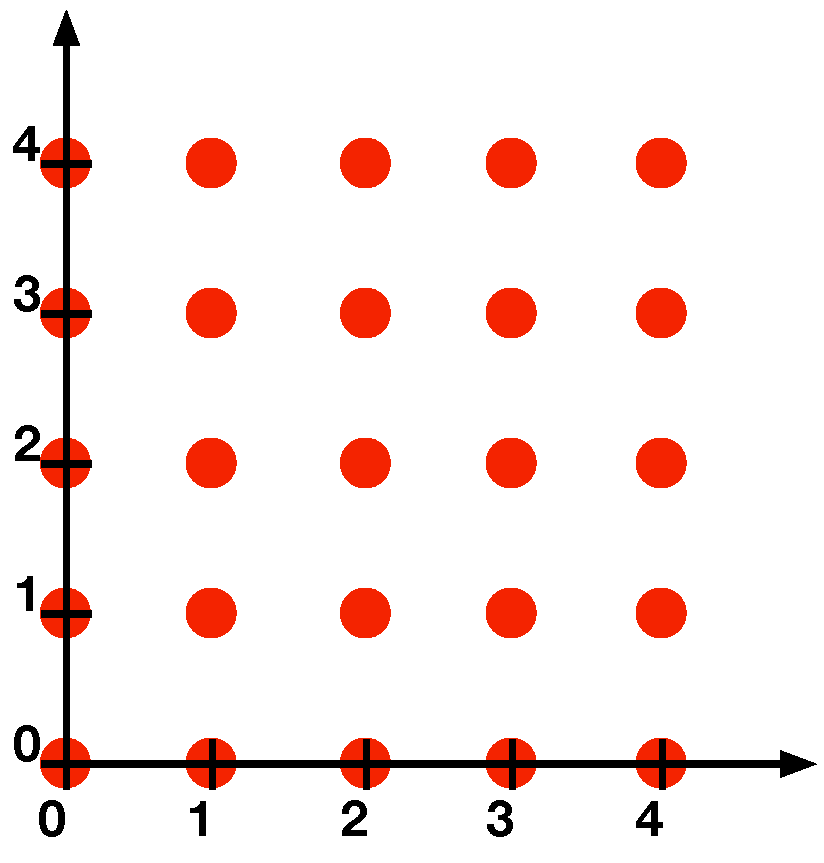
\includegraphics[width=0.5\textwidth]{GridPoints.pdf}
\caption{Grid points are illustrated as red circles though their ``physical extent'' is infinitesimally small.}
\label{fig:GridPoints}
\end{center}
\end{figure}

Next, define {\bf grid cells} as the unit partition of space into regions closest to the grid points. In other words, we define the set of grid cells as the Voronoi diagram of the grid points (in an infinitely large grid)!  Figure~(\ref{fig:CellsNodes}.a) illustrates the grid cells as green squares \emph{centered} around the $5\times5$ grid points. Unlike grid points, grid cells have a ``physical extent'' with the area $1\times1$ units.

\begin{figure}[ht]
\begin{center}
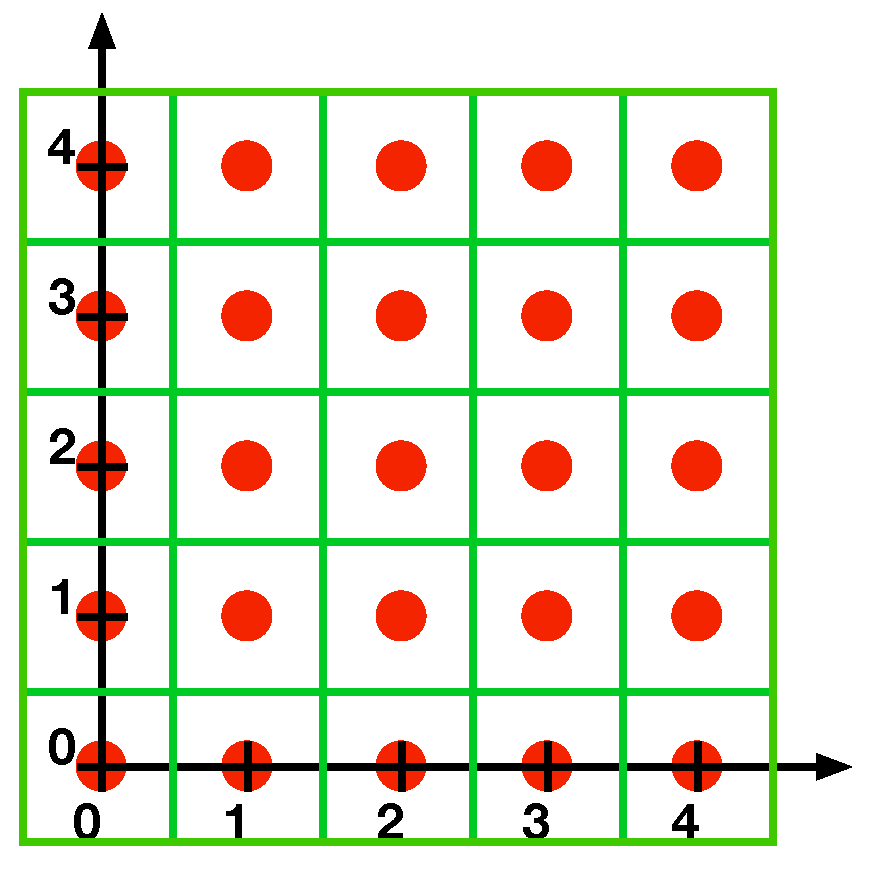
\includegraphics[width=0.50\textwidth]{GridCells.pdf}
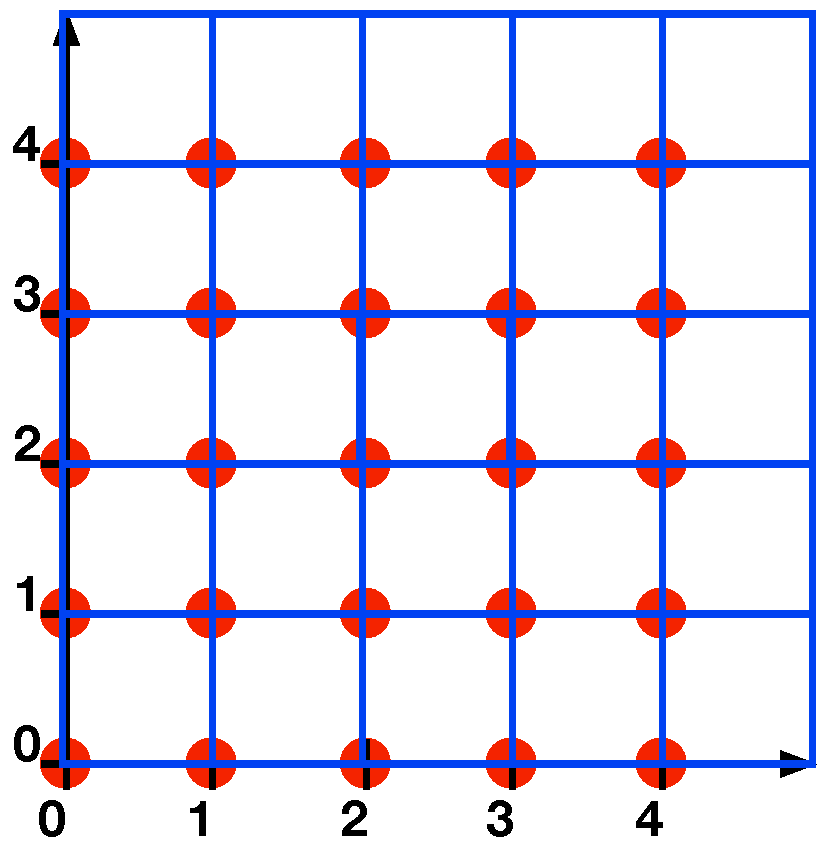
\includegraphics[width=0.48\textwidth]{GridNodes.pdf}
\caption{{\bf Left (a)}: Green grid cell centered around the red grid points. {\bf Right (b)}: Blue grid nodes coincident with the red grid points.}
\label{fig:CellsNodes}
\end{center}
\end{figure}

Note that the grid cell associated with grid point labeled $(i,j)$ spans the float-point coordinate space $(i-0.5,j-0.5)\rightarrow(i+0.5,j+0.5)$.

Next, we define {\bf grid nodes} as unit-square partitions of the coordinate space, whose corners coincide with the grid points. We furthermore adopt the convention that the grid node is labeled with the \emph{smallest} integer coordinates of its coincident grid point, that is $(i,j)$ denotes the lower-left grid point. Thus, grid node $(i,j)$ spans the integer coordinate space $(i,j)\rightarrow(i+1,j+1)$. This is show as the blue unit-squares in figure~(\ref{fig:CellsNodes}.b).

\section{Problem statement}

In short, grid cells and grid nodes are used in different parts of the library which can lead to confusion and bugs. Specifically, this is case when rendering points, as we'll detail below.

When a VDB is used as a BVH for particles/points, e.g.\ in PointIndexGrid or PointDataGrid, it is using grid cells to define the region of influence with which to partition the points into buckets. That is, the points whose (float-point) coordinates are contained in the grid cell $(i-0.5,j-0.5)\rightarrow(i+0.5,j+0.5)$ (green unit-squares in figure~(\ref{fig:CellsNodes}.a) are associated with grid point $(i,j)$. Conversely, the Digital Differential Analyzer (DDA) in our library uses grid nodes to define the discrete ray-stepping, since this allows for integer arithmetics. In other words, rays are rasterized into the grid nodes and not grid cells! In many applications this is not an issue, but point-rendering is obviously an exception because it mixes these distinct ways of associating ``extents'' with grid points. This is illustrated in figure~(\ref{fig:CellsNodesRay}.a) where a ray, starting at the blue circle, is intersecting the green grid cells that act as buckets for the particles to be rendered. In other words, we need the intersections between the ray, shown as the black arrow, and the green grid cells containing points. However, by design the DDA computes the intersection point between the black arrow and the blue grid cells, resulting in clipping. The solution is simply to offset the origin of the ray (i.e. the blue circle) by exactly $(0.5,0.5)$ since this produces the same intersections when the offsetted ray is rasterized into grid nodes by the DDA. This is illustrated in figure~(\ref{fig:CellsNodesRay}.b), where the origin of the original ray, shown as a dotted blue circle, is offset by $(0.5,0.5)$ to the solid blue circle. Note that the resulting offset ray in figure~(\ref{fig:CellsNodesRay}.b) has the same intersections with the blue lines, i.e.\ grid nodes, as the ray in figure~(\ref{fig:CellsNodesRay}.a) has for the green lines, i.e. grid cells. Finally, note that the grid points associated with respectively the intersected grid cells and grid nodes, shown as the solid red circles with black circumferences, are exactly the same in  figures~(\ref{fig:CellsNodesRay}.a) and (\ref{fig:CellsNodesRay}.b)! This is of course a consequence of the fact a grid node by definition is labeled according to its minimum incident grid point. Thus, we conclude that by offsetting the ray by $(0.5,0.5)$ we can use the DDA to correctly identify the grid points containing points as well as compute the correct intersections points along the ray. 


\begin{figure}[htbp]
\begin{center}
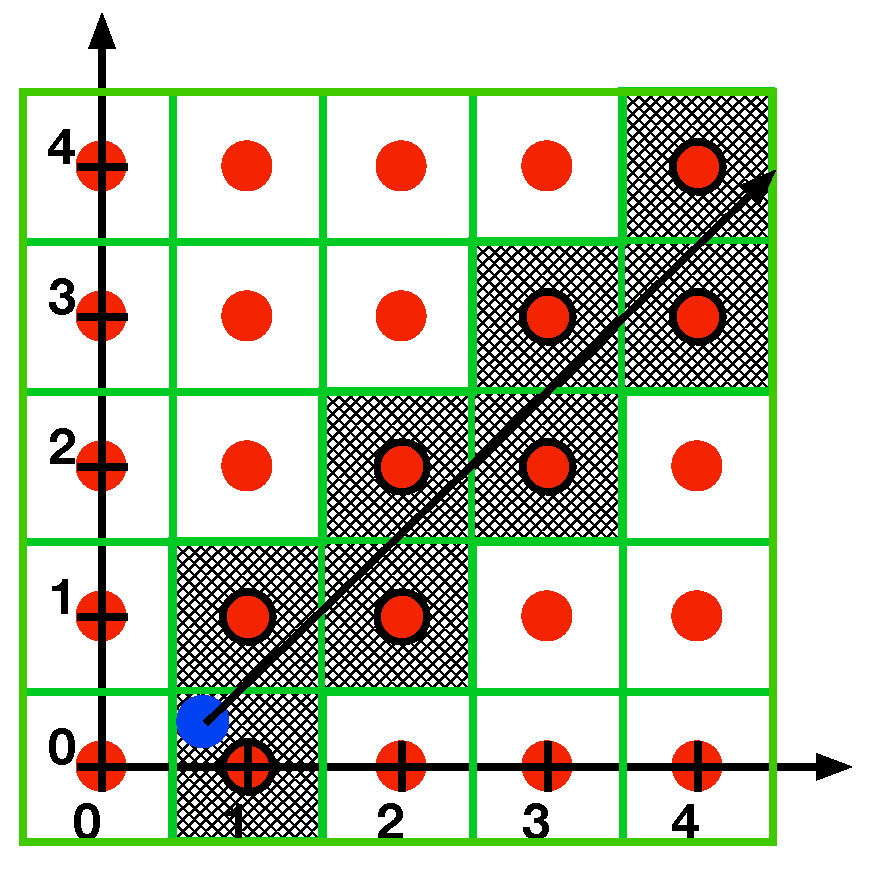
\includegraphics[width=0.50\textwidth]{GridCellsRay.pdf}
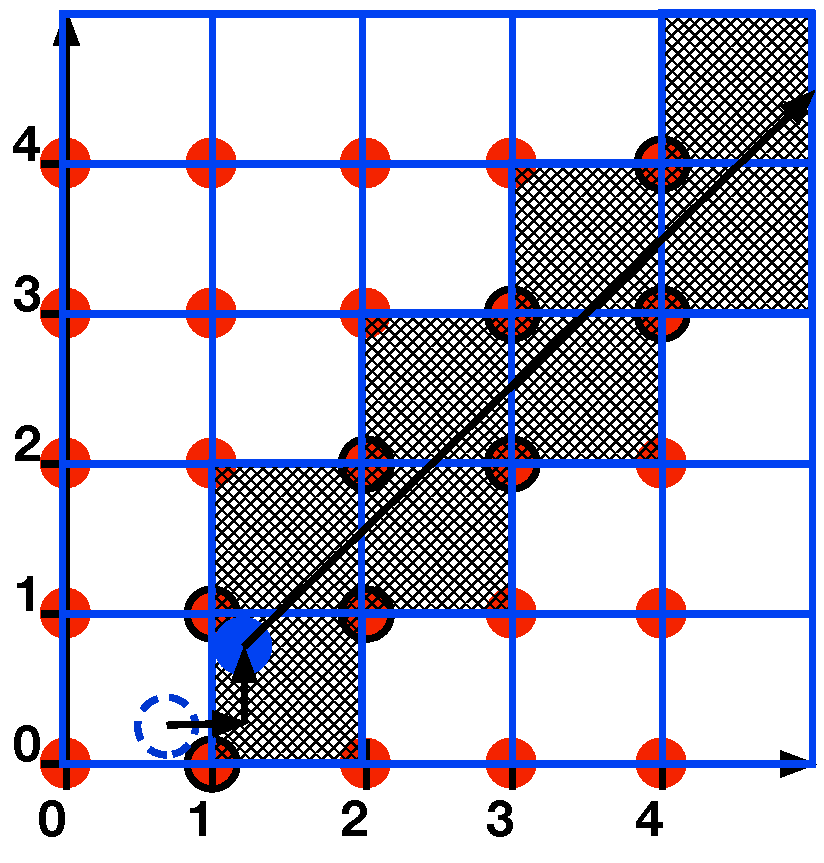
\includegraphics[width=0.48\textwidth]{GridNodesRay.pdf}
\caption{{\bf Left (a)}: Ray intersections for the green grid cells containing points. {\bf Right (b)}: Ray is offset by $(0.5,0.5)$ and intersected with the blue grid nodes.}
\label{fig:CellsNodesRay}
\end{center}
\end{figure}

\end{document}
